%%=============================================================================
%% Analyse marketing Kriket
%%=============================================================================

\chapter{Growth hack toegepast op Kriket}
\label{ch:implementatie}

Het voorbeeld dat in het vorige hoofdstuk aangehaald wordt zal hier worden uitgewerkt. Zo kan men bewijzen dat het toepassen van growth hacking kan op niet-technologische bedrijven mogelijk is. 

Het referral systeem, genaamd Referral Candy, zal in de website van Kriket (\href{https://kriket.be}{kriket.be}) worden geïmplementeerd. Dit gebeurt in samenhang van het lanceren van een nieuw product, de \emph{discover box}.

\section{Stappenplan}
\label{sec:implementatie-stappenplan}

Het stappenplan voor deze specifieke implementatie is als volgt:

\begin{enumerate}
	\item Huidige situatie bekijken
	\item Google Analytics opzetten
	\item Referral Candy toevoegen aan de Shopify website
	\item Aanpassingen aan de webshop
	\item Growth hack online zetten
	\item Monitoring gedurende één maand
	\item Data analyseren: A/B test, verkoopcijfers, aantal bezoekers, enz.
	\item Conclusie: growth hack succesvol?
\end{enumerate}

Deze worden stap voor stap uitgeschreven op de volgende pagina's. 

\subsection{Huidige situatie bekijken} \label{sec:huidige-situatie-analyseren}

Hieronder staat een overzicht van de gebruikte technologieën en platformen.

\textbf{Webshop}
\begin{itemize}
	\item Shopify
\end{itemize}

\textbf{Data en analytics}
\begin{itemize}
	\item Shopify Analytics
\end{itemize}

\textbf{Sociale media platformen}
\begin{itemize}
	\item Facebook
	\item Instagram
\end{itemize}

Dit is een goede basis waaraan Google Analytics binnen \emph{Data en analytics} wordt toegevoegd en aan de webshop wordt de module voor het referral systeem toegevoegd.

\subsection{Google Analytics opzetten} \label{sec:google-analytics-opzetten}
Het koppelen van de Shopify website met Google Analytics is een eenvoudig proces. De Google account van Kriket werd gebruikt om een Analytics profiel aan te maken. De basis-koppeling stond klaar, maar Analytics werd nog niet ten volle gebruikt. Er waren geen doelen ingesteld en zo kan men moeilijk opvolgen wat de gebruikers op de website doen. Zodra de doelen zijn ingesteld kan men specifieke acties volgen en bekijken wanneer de gebruiker stopt in het proces van betaling.

De volgende doelen werden aangemaakt:
\begin{itemize}
	\item Added address
	\item Added payment info
	\item Added product to cart
	\item Added shipping info
	\item Checkout page
	\item Order completed
\end{itemize}

\subsection{Referral Candy toevoegen} \label{sec:referral-candy-toevoegen}
De Shopify applicatie Referral Candy wordt toegevoegd en geconfigureerd naar de noden van Kriket. Het volgende concept wordt toegepast:

\emph{Arno} is heel tevreden van Kriket en wil het product aanraden aan zijn vriendin \emph{Bonnie}. Bonnie krijgt volgende URL van Arno opgestuurd via Facebook Messenger ``https://kriket.refr.cc/arno``. Bonnie is geïnteresseerd in het concept van Kriket en koopt via de link van Arno een discover box. Door de link van Arno te gebruiken heeft Bonnie 20\% kunnen besparen. Arno krijgt op zijn beurt ook voordeel en ontvangt 20\% korting op zijn volgende aankoop via een kortingscode die hij per mail krijgt opgestuurd.

Concreet gaat het als volgt in werking. De klant maakt kennis met het referral programma via:
\begin{itemize}
	\item Social media post met landingspagina (\href{https://kriket.referralcandy.com}{https://kriket.referralcandy.com})
	\item Pop-up na betaling
	\item E-mail die na aankoop wordt verstuurd
\end{itemize}
Indien de link werd aangemaakt en gedurende 2 weken niet gebruikt werd, krijgt de klant een vriendelijke reminder e-mail met de boodschap om 20\% korting niet te laten vliegen.

Vanuit Referral Candy is er ook een nieuwe koppeling met Analytics toegevoegd. Een nieuwe \emph{property} genaamd ``Referral Program``, een \emph{property} is een onderdeel van een Analytics account. Een property kan een website, mobiele applicatie of dergelijke zijn. In dit geval is Referral Candy onze nieuwe applicatie die we koppelen aan de account. Deze staat dus los van de andere property, ``www.kriket.be``, die de eerder vermelde doelen bevat. Ze ontvangen de data van andere bronnen, de ene van Shopify en de andere van Referral Candy.

\subsection{Aanpassingen aan de webshop} \label{sec:aanpassingen-webshop}
Er worden 2 producten toegevoegd aan de webshop. ``DISCOVERY BOX LARGE`` en ``DISCOVERY BOX SMALL``, deze worden gebruikt bij het referral-programma.


\begin{figure}[h!]
	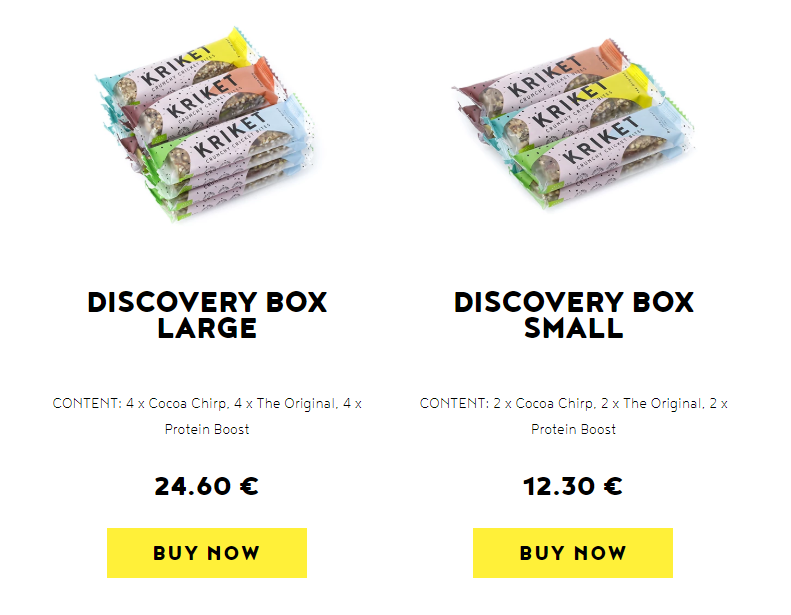
\includegraphics[width=\linewidth]{img/discovery-box-webshop.png}
	\caption{De twee nieuwe producten in de webshop.}
	\label{fig:discovery-box-webshop}
\end{figure}

Naast deze nieuwe producten toe te voegen worden de afbeeldingen verkleind. Het kleiner maken van de afbeeldingen zorgt voor een snellere laadtijd en een fijnere surf-ervaring op de webshop. Bij sommige producten is het verschil in bestand-grootte enorm - van 800Kb naar 100Kb. Tot wel 8 keer kleiner, het is een verschil dat zeker op valt.

\subsection{Growth hack online zetten} \label{sec:growth-hack-online-zetten}
Zodra het opzetten van alle voorgaande tools getest is kan de growth hack online gezet worden. Hierbij worden de twee sociale media platformen gebruikt. Langs Instagram en Facebook komen de fans en klanten van Kriket te weten dat het referral systeem beschikbaar is. Indien ze de beloning voldoende vinden en dat deze de moeite waard is, zullen ze het wellicht gebruiken. 

\subsection{Monitoring gedurende één maand} \label{sec:monitoring-gedurende-twee-weken}
Nu dat de growth hack online staat kan Google Analytics gebruikt worden voor de monitoring van deze growth hack. Hieruit zal blijken hoe vaak het referral systeem gebruikt wordt, indien blijkt dat het niet werkt zal men de beloning moeten verhogen of bijsturen op een ander gebied.

\subsection{Data analyseren} \label{sec:data-analyseren}
De data uit Google en Shopify Analytics zegt ons het volgende:

Van 26 juli tot 20 augustus

*grafiek*

A/B test, verkoopcijfers, aantal bezoekers, enz.



\subsection{Conclusie: growth hack succesvol?} \label{sec:conclusie-growth-hack-succesvol}
De conclusie.
